% Input matrix X^(0): N token columns, each a D-dimensional feature vector.
% Build:  latex input-matrix.tex && dvisvgm --no-fonts input-matrix.dvi -o input-matrix.svg
\documentclass[tikz,border=6pt]{standalone}
\usepackage[T1]{fontenc}
\usepackage{amsmath,bm}
\usetikzlibrary{arrows.meta,calc,positioning,decorations.pathreplacing}

\begin{document}
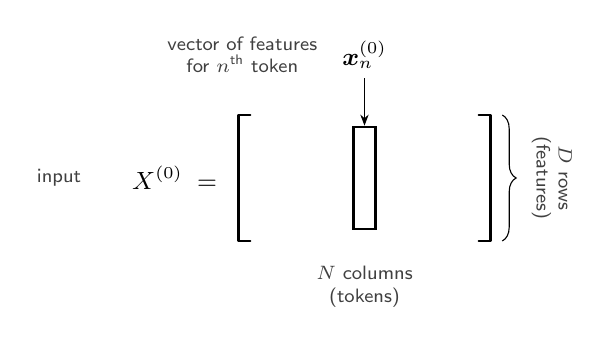
\begin{tikzpicture}[
  font=\sffamily\small,
  note/.style={font=\sffamily\scriptsize, align=center, text=black!75},
  bracket/.style={thick, line cap=round, line join=round},
]
  % ---- Matrix geometry ----------------------------------------------------
  \def\W{3.2}   % matrix width
  \def\H{1.6}   % matrix height
  \def\T{0.15}  % length of the bracket ticks

  % Square brackets
  \draw[bracket] (\T,0)    -- (0,0)  -- (0,\H)  -- (\T,\H);
  \draw[bracket] (\W-\T,0) -- (\W,0) -- (\W,\H) -- (\W-\T,\H);

  % A single column: the feature vector of one token
  \node[draw, thick, minimum width=0.28cm, minimum height=1.3cm, inner sep=0]
    (col) at (\W/2, \H/2) {};

  % ---- Left-hand side -----------------------------------------------------
  \node[anchor=east] (eq) at (-0.15, \H/2) {$X^{(0)} \;=$};
  \node[note, anchor=east] at ($(eq.west) + (-0.4, 0)$) {input};

  % ---- Annotation above: arrow to the column ------------------------------
  \node[above=0.6cm of col] (xn) {$\bm{x}_n^{(0)}$};
  \draw[-{Stealth[length=4pt]}, thin] (xn.south) -- (col.north);
  \node[note, left=2pt of xn] {vector of features\\for $n^{\text{th}}$ token};

  % ---- Annotation below: number of columns --------------------------------
  \node[note, anchor=north] at (\W/2, -0.2) {$N$ columns\\(tokens)};

  % ---- Annotation right: brace + rotated label ----------------------------
  \draw[decorate, decoration={brace, amplitude=5pt}, thin]
    (\W+0.15, \H) -- (\W+0.15, 0);
  \node[note, rotate=-90, anchor=south] at (\W+0.4, \H/2) {$D$ rows\\(features)};
\end{tikzpicture}
\end{document}
